Frevia is delivered by a single cross-functional team of five members rather than by separate frontend, backend, and testing groups. Each member holds a primary role, listed in Section 3.2, and takes one or more secondary roles for the duration of a sprint. The team leader acts as Product Owner and is accountable for the backlog order and for accepting each increment; the same member facilitates the Scrum events, so that the plan and the delivery cannot drift apart without being noticed.

The structure is deliberately flat. There is no separate quality department: the member who implements an item is also responsible for its unit tests, and the reviewer of the pull request is responsible for confirming that the Definition of Done in Section 2.1 was respected. Test ownership rotates between sprints so that each member has reviewed at least one module they did not write before the acceptance milestone.

Two interfaces sit outside the team. The project supervisor reviews the increment at the end of every sprint, provides feedback on the scope and on the documentation, and approves the submission of each report. Prospective users participate in acceptance testing in the final sprint, but they do not join sprint planning and do not negotiate scope directly with the team; their feedback reaches the backlog through the Product Owner.

\begin{figure}[H]
\centering
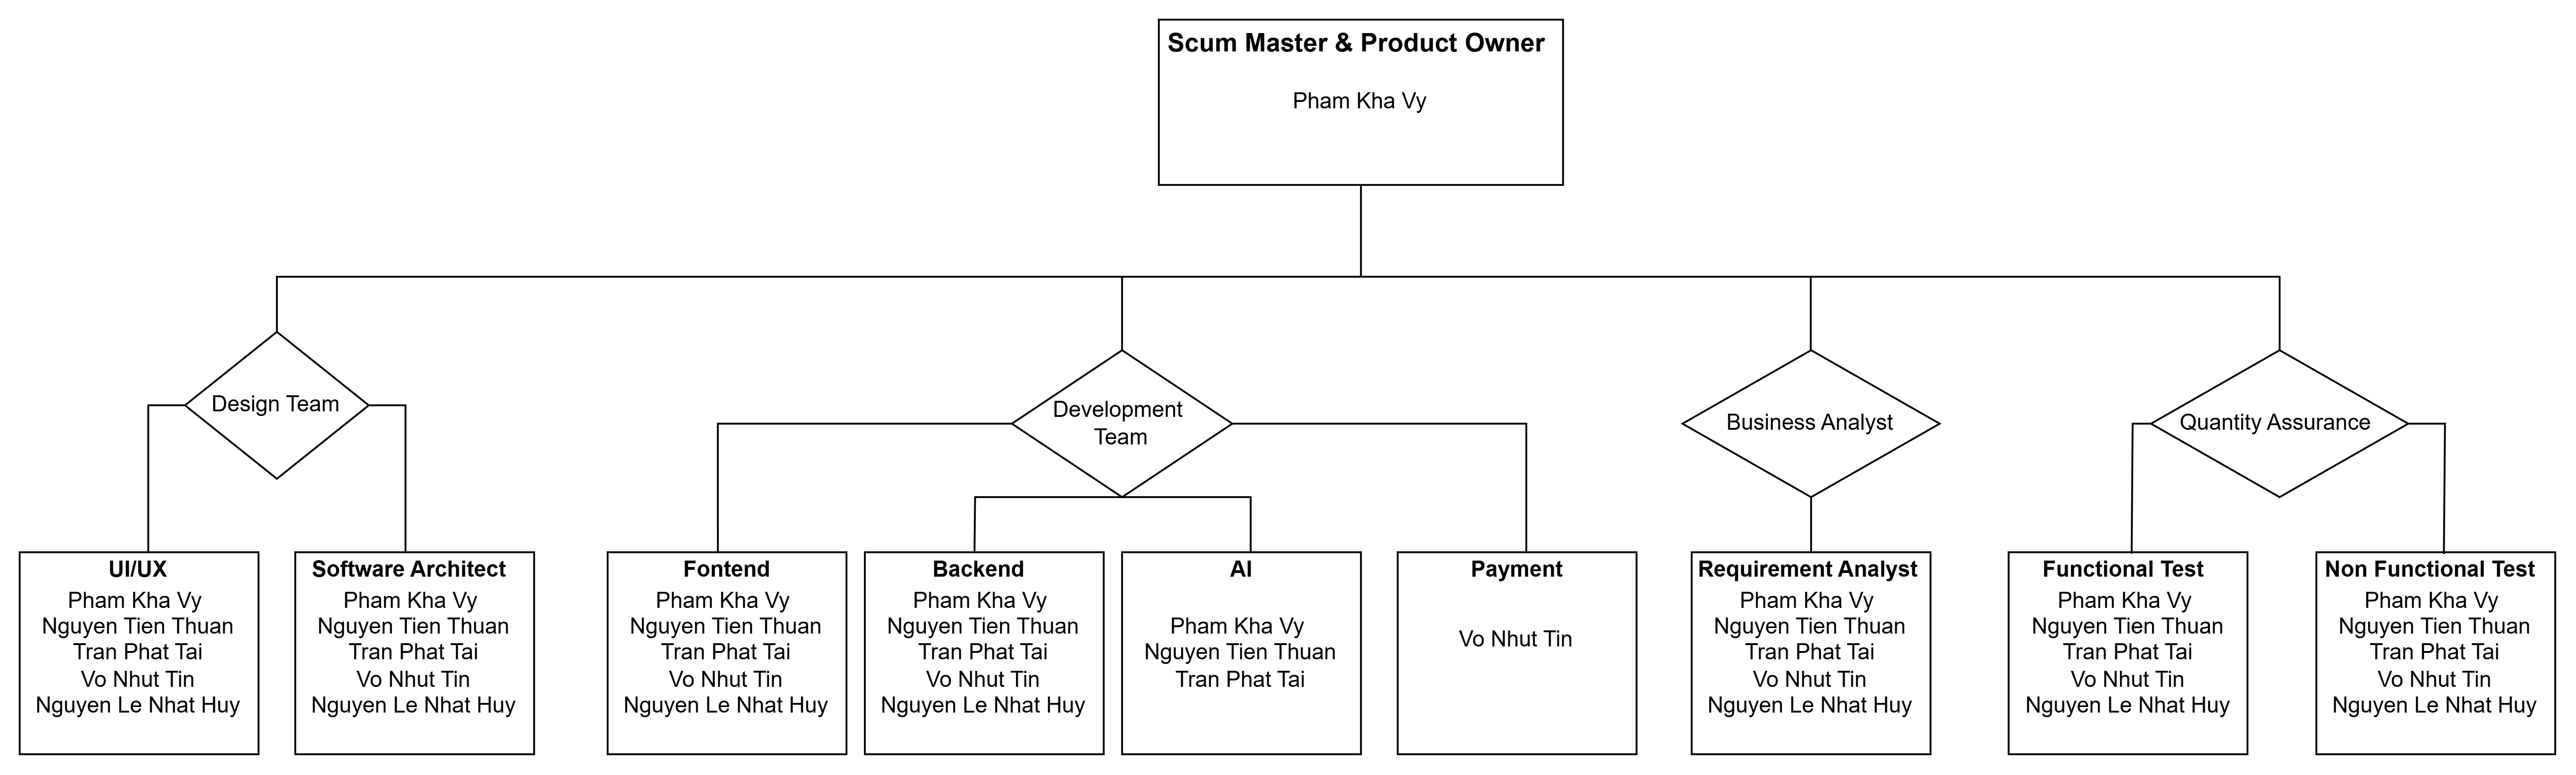
\includegraphics[width=0.8\textwidth]{team-structure.jpg}
\caption{Team and Structure Diagram}
\label{fig:team-structure}
\end{figure}
